\documentclass[11pt]{article}
\usepackage[utf8]{inputenc}
\usepackage{amsmath, amssymb}
\usepackage{graphicx}
\usepackage{hyperref}
\usepackage{geometry}
\usepackage[backend=biber]{biblatex}
\addbibresource{../references.bib}
\geometry{margin=1in}

\title{Expanding Entropy and the Birth of Spacetime}
\author{Juha Meskanen}
\date{2021}

\begin{document}
\maketitle

\begin{abstract}
   We explore the hypothesis that the growth of entropy in a computable execution trace corresponds to the expansion of spacetime, offering a natural explanation for the low-entropy initial state of the universe and its inflationary growth. Using bitstring evolution and geometric decoding rules, we demonstrate how entropy increase leads to emergent structure — from elementary particles to molecules — with their statistical frequency following a lognormal distribution.

   Unlike traditional models in General Relativity and Quantum Mechanics, we propose that the universe began in a zero-entropy state — incapable of encoding structure, and therefore devoid of curvature or gravity. As entropy increases, complexity and geometry emerge. This framework implies that the curvature at the singularity is not infinite, but identically zero — a conclusion with profound implications for the informational foundations of physics.
\end{abstract}


\section{Introduction}

This work is the third in a sequence of studies exploring the hypothesis that physical reality is fundamentally informational. In \textbf{Paper 1}, we argued that conscious observers can be described as axiomatic systems, and that time is an emergent property of the observer’s internal state transitions. \textbf{Paper 2} then applied this framework to spacetime collapse, proposing that black hole singularities correspond to points of zero entropy in an informational execution trace.

In this paper, we reverse the arrow of time: rather than studying gravitational collapse, we investigate how the \textit{increase} of entropy within a bitstring-based computational model gives rise to emergent geometric complexity — a model of spacetime birth.


\section{Entropy as a Driver of Expansion}

We define an execution trace ${S_t}_{t=0}^n$, where each $S_t$ is a binary string of fixed length $L$.
Starting from a state of zero entropy (all-zero string), we evolve $S_t$ forward using a random bit-flip mutation process that
incrementally increases entropy.

Each $S_t$ is interpreted geometrically through a decoding scheme $D: \{0,1\}^L \to \mathbb{R}^d$. In this study,
we define the hierarchy of elementary structures as follows:

1. **Spacetime fabric:** Directly defined by 3D points encoded from the bitstrings through the decoding scheme.

2. **Elementary Particles:** These are defined as pairs of 3D points, i.e., pairs of
coordinates $((x_1, y_1, z_1), (x_2, y_2, z_2))$, where the spatial separation between the
points is fixed. Specifically, an elementary particle is formed when two points in the 3D space are within
a certain threshold distance, indicating that they can be considered a pair of interacting points.

3. **Atoms:** We define an atom as a set of three points $(p_1, p_2, p_3)$ where the distances between the points satisfy:
\[
   0 < \text{distance}(p_1, p_2) < \text{threshold}, \quad 0 < \text{distance}(p_2, p_3) < \text{threshold}, \quad 0 < \text{distance}(p_3, p_1) < \text{threshold},
\]
and the distances are sufficiently close to each other such that the structure is nearly equilateral

4. **Molecules:** A molecule is formed when two atoms are sufficiently close in space, with the distance between
their centers being below a given threshold. The center of an atom is defined as the geometric center of the three points forming the atom:
\[
   \text{center}(atom) = \left( \frac{x_1 + x_2 + x_3}{3}, \frac{y_1 + y_2 + y_3}{3}, \frac{z_1 + z_2 + z_3}{3}, \frac{t_1 + t_2 + t_3}{3} \right).
\]
A molecule is considered to be formed when the distance between the centers of two atoms, $atom_1$ and $atom_2$, is below a threshold value:
\[
   \text{distance}(\text{center}(atom_1), \text{center}(atom_2)) < \text{threshold}.
\]
Thus, a molecule is a structure consisting of two atoms in close proximity, representing the next level of complexity in the hierarchy.


We define a decoding rule that extracts these particles from substrings of $S_t$, and count the number of distinct particles
present at each timestep. We simulate the evolution of $S_t$ by applying random bit flips, which increase the Shannon entropy of the string.
We find:

\begin{enumerate}
   \item Initially, when entropy is near zero, no valid particles are decoded.
   \item As entropy increases, particle count grows exponentially.
   \item This exponential rise slows as entropy increases further, matching the inflationary burst followed by slower expansion.
\end{enumerate}



\section{Statistical Properties: Lognormal Emergence}

Plotting the number of valid geometric interpretations (particles, atoms, molecules) against entropy yields a distribution resembling a lognormal curve.  The results also show that at lower entropy, only elementary particles exist, while at higher entropy, atoms and molecules emerge. This aligns with observed cosmic evolution: inflation (early burst), structure formation, and degeneration during late-time when the entropy reaches its maximum. The simulation also demonstrate natural progression from simple to complex forms as entropy increases.

This lognormal emergence mirrors statistical patterns observed in astrophysical data — such as the distribution of galaxy masses, luminosities, and star formation rates — suggesting that the informational substrate may underlie both micro and macro structure formation.


\begin{figure}[h!]
   \centering
   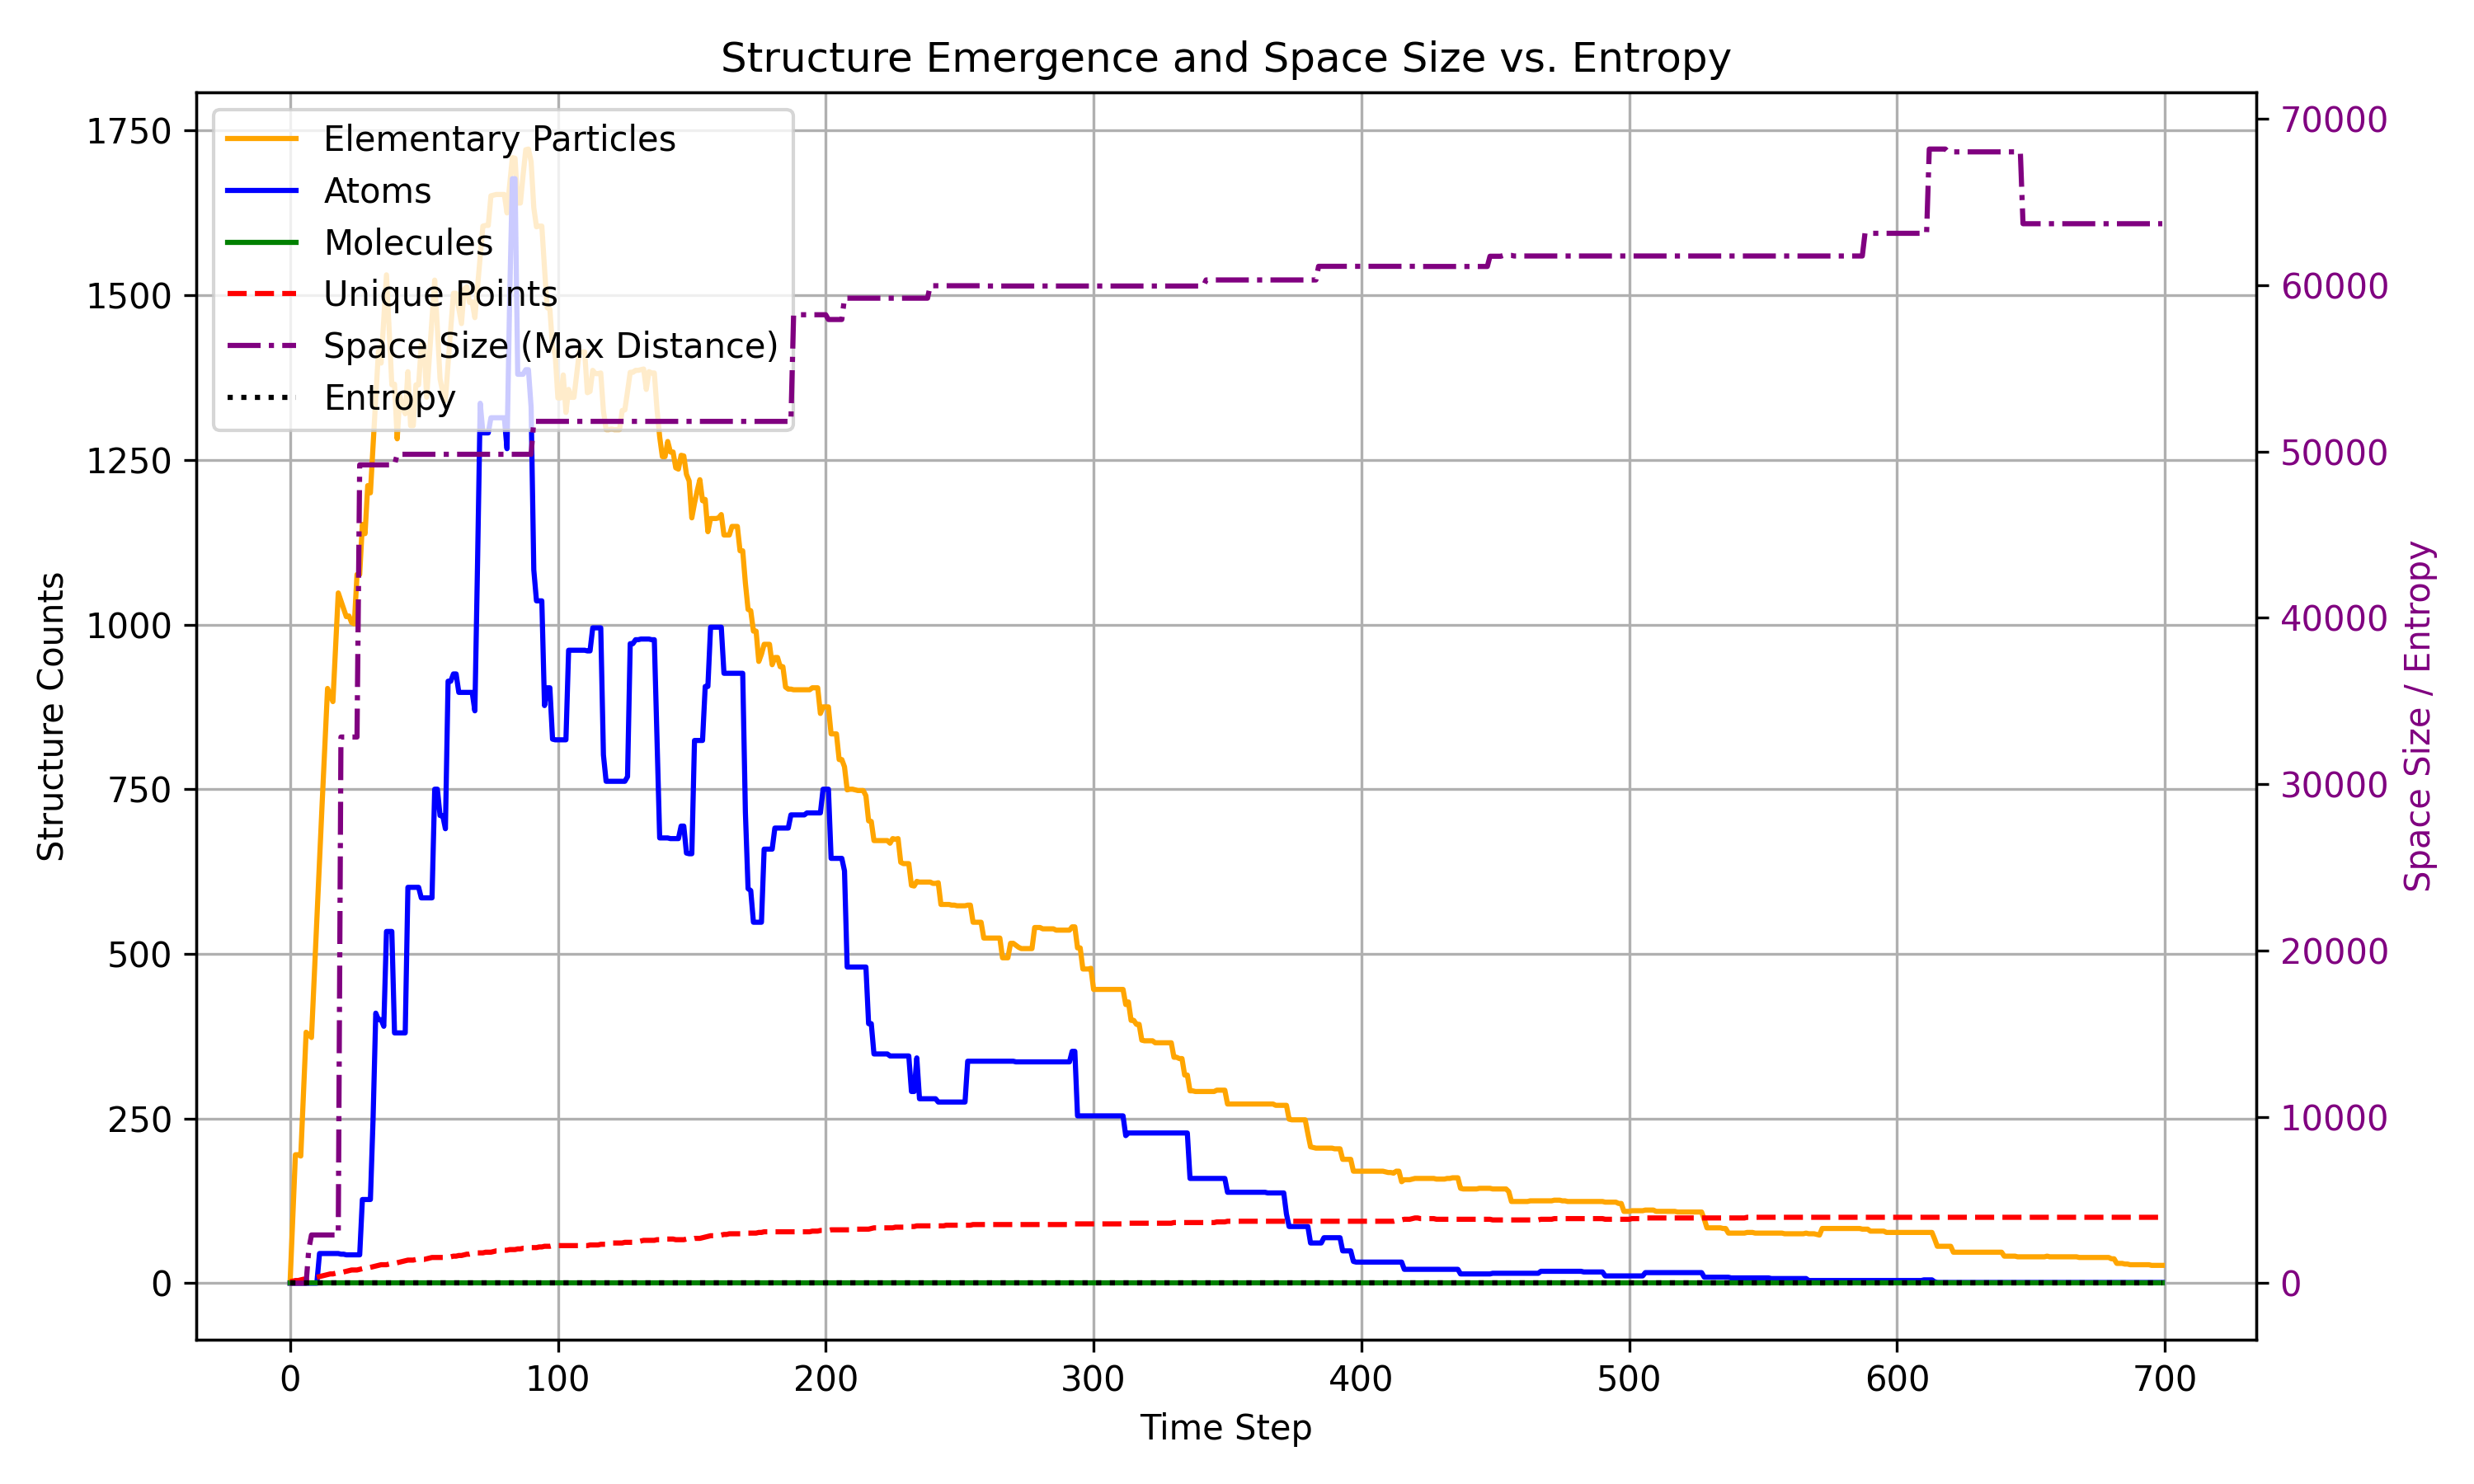
\includegraphics[width=0.8\textwidth]{figures/entropy_to_matter.png}
   \caption{Emergence of hierarchical structures in the execution trace. The emergence follows a lognormal-like distribution.}
   \label{fig:lognormal-structure}
\end{figure}

The simulation program is hosted at \url{http://github.com/juhakm/emergence_of_spacetime.py}.


\section*{Implications for Spacetime Geometry}

Although our simulation makes minimal physical assumptions and does not include traditional dynamics, it nevertheless reveals a consistent emergence of structured matter from random bitstring evolution — suggesting that informational entropy alone may be sufficient to drive the geometry of spacetime.

This statistical regularity has direct geometric implications: it suggests that the probability of matter — interpreted here as persistent, compressible patterns — is correlated with entropy. Near the entropy minimum, where the informational configuration consists of long, uniform bitstrings (e.g., all 0s or 1s), the probability of finding any distinguishable structure approaches zero. Without structure, there is no particle content — and therefore, no gravity.

This leads to a provocative conclusion: the curvature of spacetime at the singularity is not infinite, as predicted by General Relativity, but zero. The singularity, in this view, is not a region of divergent geometry but a trivial state.

This interpretation stands in stark contrast to both General Relativity, which predicts infinite curvature at the singularity, and Quantum Mechanics, which typically excludes the possibility of a fully defined, zero-entropy state. Yet, in our simulation, the universe begins in precisely such a state, and coherent geometric structures emerge only as entropy increases.

The informational view suggests a radical unification: gravity, geometry, time, and quantum effects may all arise from the same fundamental source — entropy evolution in computation. In this light, spacetime is not the stage upon which information acts, but the shadow it casts.


\section{Future Work}

We will explore the implications of the observed breakdown of both GR (due to singularities) and QM (due to the assumption of nonzero entropy at origin), and construct a unified information-theoretic framework to describe phenomena attributed to spacetime curvature and quantum entanglement.

Ultimately, we aim to replace geometric and probabilistic descriptions of the universe with a single, consistent, fully self-contained model that expects no substrace beyond information itself.


\end{document}

